\documentclass[tikz,border=10pt]{standalone}
%%%<
\usepackage{verbatim}
%%%>
% \usetikzlibrary{shapes.geometric,backgrounds,
  % positioning-plus,node-families,calc}
% \tikzset{
%   basic box/.style = {
%     shape = rectangle,
%     align = center,
%     draw  = #1,
%     fill  = #1!25,
%     rounded corners},
%   header node/.style = {
%     Minimum Width = header nodes,
%     font          = \strut\Large\ttfamily,
%     text depth    = +0pt,
%     fill          = white,
%     draw},
%   header/.style = {%
%     inner ysep = +1.5em,
%     append after command = {
%       \pgfextra{\let\TikZlastnode\tikzlastnode}
%       node [header node] (header-\TikZlastnode) at (\TikZlastnode.north) {#1}
%       node [span = (\TikZlastnode)(header-\TikZlastnode)]
%         at (fit bounding box) (h-\TikZlastnode) {}
%     }
%   },
%   hv/.style = {to path = {-|(\tikztotarget)\tikztonodes}},
%   vh/.style = {to path = {|-(\tikztotarget)\tikztonodes}},
%   fat blue line/.style = {ultra thick, blue}
% }
\begin{document}
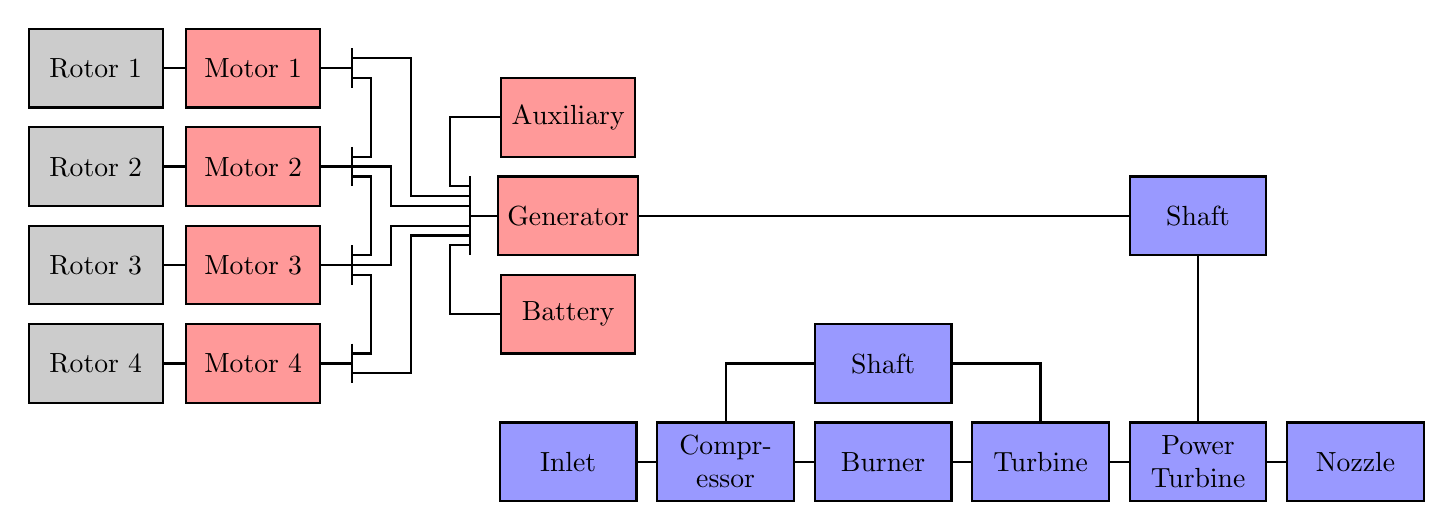
\begin{tikzpicture}[node distance = 1.2cm, thick, nodes = {align = center}, >=latex]

  \tikzstyle{rotor}=[draw, rectangle, minimum height=1cm, minimum width=1.7cm, fill=gray!40,]
  \tikzstyle{elec}=[draw, rectangle, minimum height=1cm, minimum width=1.7cm, fill=red!40,]
  \tikzstyle{cycle}=[draw, rectangle, minimum height=1cm, minimum width=1.7cm, text width=1.5cm, fill=blue!40,]

  
  % \node[rotor] (r1) at (0,0) {Rotor 1};
  % \node[rotor] (r2) at (2,0) {Rotor 2};
  % \node[rotor] (r3) at (4,0) {Rotor 3};
  % \node[rotor] (r4) at (6,0) {Rotor 4};

  % \node[elec] (m1) at (0,-1.5) {Motor 1};
  % \node[elec] (m2) at (2,-1.5) {Motor 2};
  % \node[elec] (m3) at (4,-1.5) {Motor 3};
  % \node[elec] (m4) at (6,-1.5) {Motor 4};

  % \node[elec] (gen) at (3,-4.5) {Generator};

  % \node[cycle] (comp) at (3,-5.5) {Compressor};
  % \node[cycle] (burn) at (3,-6.5) {Burner};
  % \node[cycle] (turb) at (3,-7.5) {Turbine};
  % \node[cycle] (pt) at (3,-8.5) {Power Turbine};
  % \node[cycle] (nozz) at (3,-9.5) {Nozzle};
  % \node[cycle] (shaft) at (5,-6.5) {Shaft};


  % Prop/rotor
  \node[rotor] (r1) at (0,5.00) {Rotor 1};
  \node[rotor] (r2) at (0,3.75) {Rotor 2};
  \node[rotor] (r3) at (0,2.50) {Rotor 3};
  \node[rotor] (r4) at (0,1.25) {Rotor 4};

  % Electrical
  \node[elec] (m1) at (2.0,5.00) {Motor 1};
  \node[elec] (m2) at (2.0,3.75) {Motor 2};
  \node[elec] (m3) at (2.0,2.50) {Motor 3};
  \node[elec] (m4) at (2.0,1.25) {Motor 4};
  \node[elec] (aux) at (6,4.375) {Auxiliary};
  \node[elec] (gen) at (6,3.125) {Generator};
  \node[elec] (batt) at (6,1.875) {Battery};

  % Cycle
  \node[cycle] (inlet) at (6,0) {Inlet};
  \node[cycle] (comp) at (8,0) {Compr-essor};
  \node[cycle] (burn) at (10,0) {Burner};
  \node[cycle] (turb) at (12,0) {Turbine};
  \node[cycle] (pt) at (14,0) {Power Turbine};
  \node[cycle] (nozz) at (16,0) {Nozzle};
  \node[cycle] (hp_shaft) at (10,1.25) {Shaft};
  \node[cycle] (lp_shaft) at (14,3.125) {Shaft};

  % Buses
  \draw (3.25,5.25) -- (3.25,4.75);
  \draw (3.25,4.0) -- (3.25,3.5);
  \draw (3.25,2.75) -- (3.25,2.25);
  \draw (3.25,1.5) -- (3.25,1.0);
  % \draw (4.75,4.125) -- (4.75,4.625);
  \draw (4.75,2.625) -- (4.75,3.625);
  % \draw (4.75,1.625) -- (4.75,2.125);

  % Lines between rotors and motors
  \draw (r1) -- (m1);
  \draw (r2) -- (m2);
  \draw (r3) -- (m3);
  \draw (r4) -- (m4);

  % Lines between motors and buses
  \draw (m1) -- (3.25,5.0);
  \draw (m2) -- (3.25,3.75);
  \draw (m3) -- (3.25,2.5);
  \draw (m4) -- (3.25,1.25);

  % Lines between generator and bus
  \draw (gen) -- (4.75,3.125);

  % Lines between batt/aux and bus
  % \draw (aux) -- (4.75,4.375);
  % \draw (batt) -- (4.75,1.875);

  % Lines for cross wing cables
  \draw (3.25,1.25+0.125) -- (3.5,1.25+0.125) -- (3.5,2.5-0.125) -- (3.25,2.5-0.125);
  \draw (3.25,2.5+0.125) -- (3.5,2.5+0.125) -- (3.5,3.75-0.125) -- (3.25,3.75-0.125);
  \draw (3.25,3.75+0.125) -- (3.5,3.75+0.125) -- (3.5,5.0-0.125) -- (3.25,5.0-0.125);


  % Lines for major cables
  \draw (3.25,1.25-0.125) -- (4.0,1.25-0.125) -- (4.0,3.125-0.25) -- (4.75,3.125-0.25);
  \draw (3.25,5.0+0.125) -- (4.0,5.0+0.125) -- (4.0,3.125+0.25) -- (4.75,3.125+0.25);

  \draw (3.25,2.5) -- (3.75,2.5) -- (3.75,3.125-0.125) -- (4.75,3.125-0.125);
  \draw (3.25,3.75) -- (3.75,3.75) -- (3.75,3.125+0.125) -- (4.75,3.125+0.125);

  \draw (batt) -- (4.5,1.875) -- (4.5,3.125-0.375) -- (4.75,3.125-0.375);
  \draw (aux) -- (4.5,4.375) -- (4.5,3.125+0.375) -- (4.75,3.125+0.375);


  % Lines between cycle elements
  \draw (inlet) -- (comp);
  \draw (comp) -- (burn);
  \draw (burn) -- (turb);
  \draw (turb) -- (pt);
  \draw (pt) -- (nozz);
  \draw (comp) -- (8,1.25) -- (hp_shaft);
  \draw (turb) -- (12,1.25) -- (hp_shaft);
  \draw (gen) -- (lp_shaft);
  \draw (pt) -- (lp_shaft);


  % \node[Minimum Width = loop, fill = yellow, below = of imp-sol] (rec-box)
  %   {rectangular box, and very wiiiiiiiiiiiiiiide\\2nd line};
  % \node[shift = (left:.5*x_node_dist)] at
  %   ($(imp-sol.west|-imp-sol.south)!.5!(rec-box.north west)$) (for-1)
  %   {formula 1};
  % \node[shift = (right:.5*x_node_dist)] at
  %   ($(imp-sol.east|-imp-sol.south)!.5!(rec-box.north east)$) (for-2)
  %   {formula 2};
  % \begin{scope}[on background layer]
  %   \node[fit = (for-1)(for-2)(imp-sol)(rec-box), basic box = blue,
  %     header = DMFT loop] (dmft-l) {};
  % \end{scope}
  % \path[very thick, blue, hv] (rec-box) edge[->] (for-1) edge[<-] (for-2)
  %                             (imp-sol) edge[->] (for-2) edge[<-] (for-1);

  % \node[east above = of dmft-l, basic box = green, header = DMFT prelude]
  %   (dmft-p) {Math and text math and text math and text\\
  %             math and text math and text math and text};
  % \node[north left = of dmft-l, basic box = green, header = $\rho$ update,
  %    shift = (down:y_node_dist)] (rho)
  %   {Much more text much more text\\much more text much more text};
  % \node[basic box = blue, header = DFT part, anchor = north] at
  %   (dmft-p.north-|rho) (dft) {So much text so much text so much text\\
  %   I think I need \texttt{tikz-lipsum}\\or something like that.};
  % \node[basic box = green, anchor = north] at
  %   ($(dft.north east)!.5!(dmft-p.north west)$) (upd) {update\\$math$};
  % \path[fat blue line, <-, dashed, vh] (rho) edge
  %   ({$(rho.south)!.5!(dmft-l.south)$}-|dmft-l.south west);
  % \path[fat blue line, ->]
  %   ({$(upd.south)!.5!(dmft-p.south)$}-|dmft-p.south west)
  %   coordinate (@) edge[<-, solid] coordinate[pos=.15] (@s)
  %   coordinate[pos=.9] (@e) (@-|dft.east)
  %   {[every edge/.append style=dashed, vh] (@s) edge[<-] (upd) (@e) edge (upd)}
  %   (h-rho) edge[dashed] (dft)
  %   ($(dmft-p.south)!.5!(dmft-p.south east)$)
  %   coordinate (@) edge (@|-dmft-l.north);
\end{tikzpicture}
\end{document}